\documentclass[12pt]{article}
\usepackage[english]{babel}
\usepackage[utf8x]{inputenc}
\usepackage{amsmath}
\usepackage{tikz}
\usetikzlibrary{arrows,automata}
\begin{document}

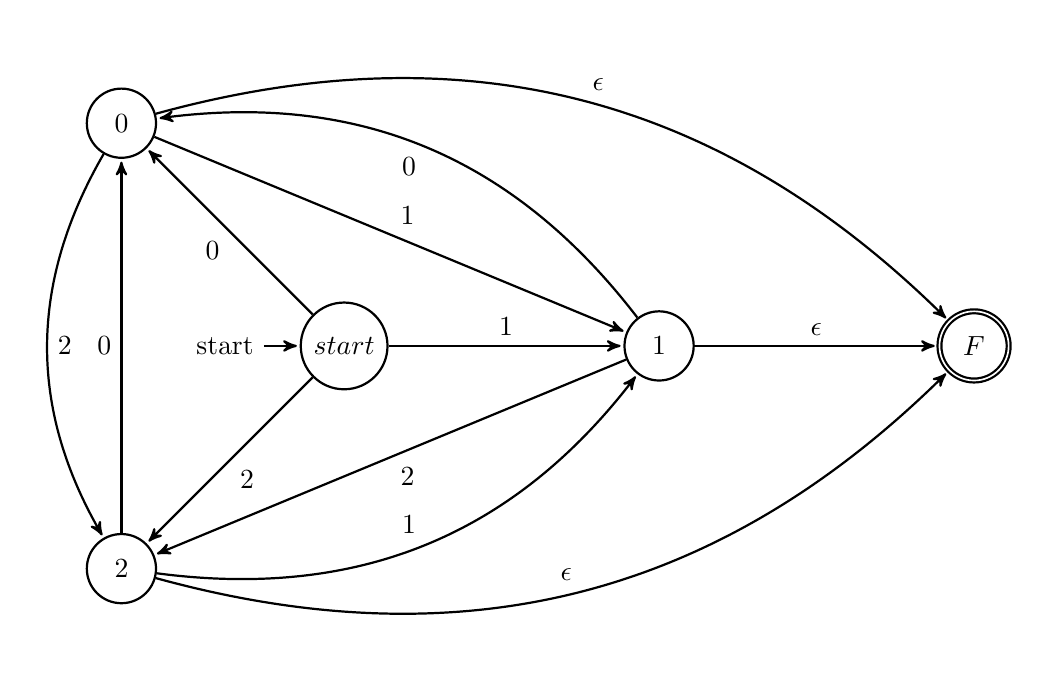
\begin{tikzpicture}[->,>=stealth',shorten >=1pt,auto,node distance=4cm,
    thick,base node/.style={circle,draw,minimum size=8pt}, real node/.style={double,circle,draw,minimum size=17pt}]

  \node[state,initial] (start) {$start$};
  \node[state] (0) [above left of=start] {$0$};
  \node[state] (1) [right of=start] {$1$};
  \node[state] (2) [below left of=start] {$2$};
  \node[state,accepting] (F) [right of=1] {$F$};
  
  \path (start) edge              node {$0$} (0)
        (start) edge              node {$1$} (1)
        (start) edge              node {$2$} (2)
        (0) edge              node {$1$} (1)
            edge     [bend right]          node {$2$} (2)
            edge [bend left] node {$\epsilon$} (F)
        (1) edge   [bend right]          node {$0$} (0)
         edge               node {$2$} (2)
         edge  node {$\epsilon$} (F)
        (2) edge                node {$0$} (0)
         edge     [bend right]         node {$1$} (1)
         edge [bend right] node {$\epsilon$} (F)
         ;

\end{tikzpicture}
\end{document}